\section{\uppercase{Background}}
This section highlights the BPMax algorithm, summarizes the polyhedral model, and then describes the code-generation technique using \alphaz\ .

\subsection{\uppercase{BPMax ALGORITHM}}
BPMax uses weighted base-pair counting for base-pair maximization. It considers  both intermolecular and intramolecular
\begin{figure}[htbp]
\centerline{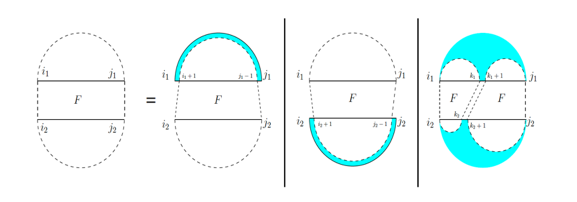
\includegraphics[scale=.9]{bpmax.png}}
\caption{The four cases defining table $F$}
\label{fig:bpm_eddy_rivas}
\end{figure}
\begin{equation}
\label{eqn:bpm_recurrence}
F_{i_{1},j_{1}, i_{2}, j_{2}}  =max \left \{\begin{array}{lr}
                 S_{i_{2}, j_{2}}^{(2)}   \hspace{10pt} j_{1}\le i_{1} \\
                 \\
                 S_{i_{1}, j_{1}}^{(1)}   \hspace{10pt} j_{2}\le i_{2} \\
                 \\
                 \text{iscore}(i_{1}, i_{2})   \hspace{20pt}  i_{1} = j_{1} \text{ and }  i_{2} = j_{2} \\
                 \\
                 \max[ \colorboxed{brown}{F_{i_{1}+1, j_{1}-1, i_{2}, j_{2}}} + \text{score}(i_{1}, j_{1}), \\
                      \colorboxed{gray}{F_{i_{1}, j_{1}, i_{2}+1, j_{2}-1}} + \text{score}(i_{2}, j_{2}), \\
                      H_{i_{1},j_{1},i_{2},j_{2}}]   \hspace{30pt}  otherwise
               \end{array}
           \right. \\
\end{equation}
\begin{equation}
\label{eqn:bpm_recurrence_h}
H_{i_{1},j_{1},i_{2},j_{2}} \\ = \max \left \{\begin{array}{lr}
                 S^{(1)}(i_{1}, j_{1})  + S^{(2)}(i_{2}, j_{2}), \\
                 \\
                \\D_{i_{1},j_{1},i_{2},j_{2}}\\
                 \\
                 \colorboxed{green}{\max\limits_{k_{2}=i_{2}}^{j_{2}-1} S^{(2)}(i_{2}, k_{2}) + F_{i_{1},j_{1}, k_{2}+1, j_{2}}}\\
                 \\
                 \colorboxed{orange}{{\max\limits_{k_{2}=i_{2}}^{j_{2}-1} F_{i_{1},j_{1}, i_{2}, k_{2}} + S^{(2)}(k_{2}+1, j_{2})}}\\
                 \\
                 \colorboxed{violet}{\max\limits_{k_{1}=i_{1}}^{j_{1}-1}  S^{(1)}(i_{1}, k_{1}) + F_{k_{1}+1,j_{1},i_{2}, j_{2}}}\\
                 \\
                 \colorboxed{yellow}{\max\limits_{k_{1}=i_{1}}^{j_{1}-1} F_{i_{1},k_{1}, i_{2}, j_{2}}+ S^{(1)}(k_{1}+1, j{1})} \\
               \end{array}
           \right. \\
\end{equation}
\begin{equation}
\label{eqn:bpm_recurrence_h_dmaxp1}
D_{i_{1},j_{1},i_{2},j_{2}} \\ = 
                 \colorboxed{blue}{\max\limits_{k_{1}=i_{1}}^{j_{1}-1} \max\limits_{k_{2}=i_{2}}^{j_{2}-1} F_{i_{1},k_{1}, i_{2}, k_{2}}+ F_{k_{1}+1,j_{1}, k_{2}+1, j_{2}}}\\
\end{equation}
base pairings. It does not allow pseudo-knots or crossings. Mathematically, it produces a four-dimensional triangular table - $F$-table (a triangular collection of triangles) based on two input sequences. Figure~\ref{fig:bpm_eddy_rivas} shows the main cases for the $F$-table using Eddy-Rivas diagram. Equation~\ref{eqn:bpm_recurrence},   Equation~\ref{eqn:bpm_recurrence_h}, and Equation~\ref{eqn:bpm_recurrence_h_dmaxp1} show the complete recurrence equation of BPMax. Equation~\ref{eqn:bpm_recurrence_h_dmaxp1} highlighted in the blue color represents the double max-plus operation. It is the most compute-intensive portion of the algorithm. We use the same colors to highlight the dependence pattern in section \ref{section:methods}.


\subsection{Polyhedral Model}
The Polyhedral model~\cite{sanjay-fst-tcs, quinton-jvsp89, feautrier91, feautrier92a, feautrier92b} is a mathematical framework for automatic optimization and parallelization of affine programs. A polyhedron is the intersection of finitely many half-spaces. It can be bounded (polytope) or unbounded. Static control parts like variables, iteration space (loop nests), and dependencies can be represented using polyhedra. 
\begin{lstlisting}[label={listing:scan}, language=Caml, caption={Prefix sum}]
    for(int i=0;i<7;i++ ) {
        sum[i]=0;
        for (int j=0 ; j<=i;  j++) 
            sum[i] += array[j]; 
    }
\end{lstlisting}
Let us consider the prefix sum code highlighted in Listing~\ref{listing:scan}   that computes the prefix-sum of an array of size $7$. The iteration space for this computation can be represented using the intersection of the finite half-spaces or set of inequalities such as $j \leq i$,  $i \leq 6$  and $j = 0$ .  The points in the iteration spaces are marked with the dots represented by the polyhedron with vertices - $(0, 0), (0, 6)$, and $(6, 0)$.
\begin{figure}[htbp]
\begin{adjustbox}{varwidth=\textwidth,margin=0 {\abovecaptionskip} 0 0, frame=0.00pt}
\centerline{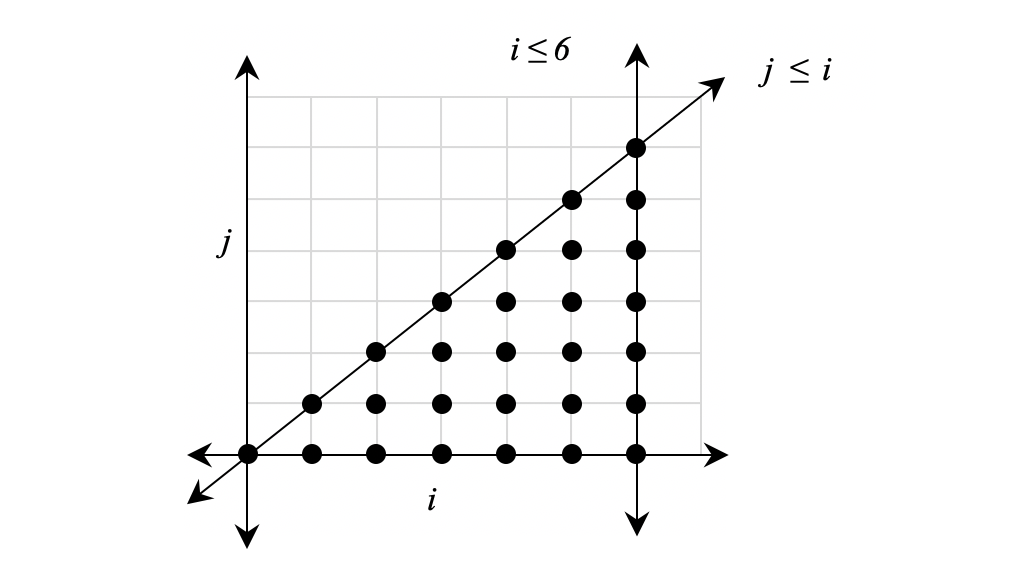
\includegraphics[scale=.48]{iteration_space.png}}
\end{adjustbox}
\caption{Polyhedral iteration space for prefix-sum}
\label{fig}
\end{figure}
The data space is usually one or more dimensions less than the iteration space. As a result, the data access functions are many-to-one mappings from iteration to data space. However, they are affine, leading to the model's clean closure properties under program transformation.

Going back to the original equation, a concise way to look at this computation would be to view it as an equation $\displaystyle sum[i] = \sum_{j=0}^{i}array[j]$.  The idea behind a polyhedral tool like \alphaz\ is exactly the reverse. It allows users to express one or more system of affine recurrence equations as a program, transform them using the polyhedral transformations that reduce the complexity of the program, use a better processor and memory allocation and then produce code for a language of interest.

\subsection{\uppercase{ALPHAZ}}
\alfa\ is a strongly typed functional language that works on a system of affine recurrence equations defined over polyhedral domains. Maurus~\cite{Mauras1989}  proposed this equational programming language as part of his doctoral dissertation.   Subsequently, it has been extended to include subsystems and reductions~\cite{leverge-thesis, leverge-parle92, fdupont-asap96, florent-thesis, DupontQuRi93}. Feautrier~\cite{feautrier91} showed that a polyhedral segment of code shown in Listing~\ref{listing:scan} can be translated to an \alfa\ program. \alfa\ is richer, mathematically cleaner, and more natural, especially, but not exclusively due to reductions.  \alphaz\ is the tool that allows program transformations and user-directed compilation of \alfa\ programs.  It provides a general framework for analysis, transformation, and code generation in polyhedral equational model.  \alphaz\ is similar to an earlier tool - \textsc{\texttt{MMAlpha}} , which targets field-programmable gate array based hardware design ~\cite{guillou-mma}. On the other hand, \alphaz\ targets code generation for multiprocessor shared-memory programs and focuses on programs with reduction operations. 

Every  \alfa\ program has two pieces – system definition and compilation script.  System definition of an  \alfa\ program allows users to express input and output of the program using polyhedral domains. 
It also allows a programmer to express the computation in terms of equations. The program containing the system definition is called alphabets. The second piece is the compilation script that contains commands to parse the input specification, transform the program based on the user input and finally generate the code. Algorithm~\ref{algo:matrix_mul_alphabets} highlights the alphabets program for matrix multiplication. Algorithm~\ref{algo:matrix_mul_script} presents a compiling script for matrix multiplication.
\begin{algorithm}
\caption{Matrix Multiplication in Alphabets}
\begin{algorithmic} [1]
\STATE \textbf{affine} MM $\lbrace N,K,M \mid (M, N, K)  > 0  \rbrace$
\STATE \textbf{input}
\STATE  \hspace{10pt} float A $\lbrace i, j \mid 0 \leq i < M \hspace{2pt} \&\& \hspace{2pt} 0 \leq j < K   \rbrace$ ;
\STATE  \hspace{10pt} float B $\lbrace i, j \mid 0 \leq i < K \hspace{2pt} \&\& \hspace{2pt} 0 \leq j < N   \rbrace$ ;
\STATE \textbf{output}
\STATE  \hspace{10pt} float C $\lbrace i, j \mid 0 \leq i < M \hspace{2pt} \&\& \hspace{2pt} 0 \leq j < N   \rbrace$;
\STATE \textbf{local}
\STATE \hspace{10pt} \slash \slash \text{local variables}
\STATE \textbf{output}
\STATE \hspace{10pt} C[$i,j$] = reduce(+, \hspace{2pt} [$k$], \hspace{2pt} A[$i,k$] * B[$k,j$]);
\end{algorithmic}
\label{algo:matrix_mul_alphabets}
\end{algorithm}
\subsubsection{Program Parsing}
The first step is to read the alphabets program, which decomposes the equations into abstract syntax tree notation internally and sets up the stage for various program transformations.
\subsubsection{Program Transformation}
All transformations in \alphaz\ are semantic preserving. However, it is the responsibility of the user to ensure the transformations are valid. \textit{Normalize} is the most basic transformation. It normalizes expression into normal form as per definition and makes the program easier to read and understand. \textit{NormalizeReduction} transforms unnormalized form to normalize form. A normal form of a reduction transforms the reduce-expression to be a direct child of an equation.  \textit{setSpaceTimeMap} allows the user to specify schedule and processor allocation to specify the order in which one or more processors visit the iteration space. A system with multiple variables requires the dimension of all the spacetime maps to be equal. \textit{NormalizeReduction} generates additional variables associated with the reductions. Specifying the schedule for such variable requires two different schedules to be provided – the first one specifies the order in which the iteration space will be visited.
 \begin{algorithm}
 \caption{Matrix Multiplication Command Script}
 \begin{algorithmic} [1]
 \STATE \text{\slash \slash \hspace{2pt}$Step-1: Parse \hspace{2pt} Alphabet \hspace{2pt} $}
 \STATE \text{prog=ReadAlphabets("MM.ab");}
 \STATE \text{system = “MM”;}
 \STATE \text{outDir="./src";}

 \STATE \text{}
 \STATE \text{\slash \slash \hspace{2pt}$Step-2: Perform \hspace{2pt} polyhedral \hspace{2pt}  transformation$}
 \STATE \text{Normalize(prog);}
 \STATE \text{setSpaceTimeMap(prog,  system,  “C”,  }
 \STATE \text{\hspace{140pt}"($i,j,k \mapsto i, k, j$)”,}
 \STATE \text{\hspace{140pt}“($i,j \mapsto i, -1, j$)”);}
 \STATE \text{setParallel(prog,  system,  “”,  "0" );}
 \STATE \text{}
 \STATE \text{\slash \slash \hspace{2pt}$Step-3: Generate  \hspace{2pt} code$}
 \STATE \text{generateWriteC(prog,  system,  outDir);}
\STATE \text{generateScheduleC(prog,  system,  outDir);}
\end{algorithmic}
\label{algo:matrix_mul_script}
\end{algorithm}
The other specifies the time at which the initialization should occur before starting the reduction. It also has a dependency on the schedule. \textit{setMemoryMap} - Memory map is a mapping between iteration points in the domain to the memory location. By default, \alphaz\ uses identity function as a memory map for each variable and bounding box of the polyhedral representation of the variable for storage. It allows multiple variables with different dimensions to share the same memory map based on affine function. \textit{setMemorySpace} is similar to memory map. Except that multiple variables with the same dimension can share memory space. \textit{setParallel} allows the user to specify one or more dimensions of the schedule to be executed in parallel by different threads. Users can also specify predicate as an ordering dimension to define the parallel loop dimension. Tiling transformation allows the user to chop the iteration space to improve data locality and adjust parallelization granularity.


\subsubsection{Code Generation}
This set of commands produce target code (e.g., c) based on the program transformation. \alphaz\ has various code generation options like – \textit{generateWriteC} which is sequential in nature and useful to check the correctness of the program, schedule code generation – \textit{generateScheduleC}. Sequential code generation hardly requires any
\begin{lstlisting}[language=Caml, caption=Generated code - Matrix multiplication]
    #define S1(i,j,i2) C(i,i2) = 0.0
    #define S0(i0,i1,i2) C(i0,i2) = (C(i0,i2))+((A(i0,i1))*(B(i1,i2)))
    {
        int c1,c2,c3;
        #pragma omp parallel for private(c2,c3)
        for(c1=0;c1 <= M-1;c1+=1){
	        for(c3=0;c3 <= N-1;c3+=1){
	            S1((c1),(-1),(c3));
	        }
            for(c2=0;c2 <= K-1;c2+=1){
                for(c3=0;c3 <= N-1;c3+=1){
                    S0((c1),(c2),(c3));
                }
            }
        }
    }
\end{lstlisting}
program transformation. However, efficient schedule code generation depends on the choice of various transformations, mainly the target mapping-related transformations. The tiling transformation is not applied upfront rather invoked as part of the post processing phase of the schedule code generation. 
%Please refer to Kim et al. \cite{Kim2010} for more details on tiling code generation algorithm.

%\Comment{Haven't read beyond this}